\subsubsection{Low Storage Runge-Kutta}

\begin{table}[!ht]
  \centering
  \caption{Oscillation test: errors analysis of explicit Low Storage Runge-Kutta solvers}\label{tab:oscillation_errors_ls_rk}
  \begin{subtable}[b]{0.40\textwidth}
    \centering
    \caption{1 stage}\label{tab:oscillation-ls-rk-1}
    \resizebox{1.00\textwidth}{!}{%
    \begin{tabular}{ccccc}
      \toprule
      {\sc Time Step} & {\sc Error X} & {\sc Error Y} & {\sc Order X} & {\sc Order Y} \\
      \hline
      5000.0          &  0.840E+10    &  0.706E+10    & /             & /             \\
      2500.0          &  0.503E+06    &  0.570E+06    & 14.03         & 13.60         \\
      1250.0          &  0.289E+04    &  0.272E+04    &  7.45         &  7.71         \\
       625.0          &  0.239E+03    &  0.232E+03    &  3.59         &  3.55         \\
       320.0          &  0.737E+02    &  0.722E+02    &  1.76         &  1.74         \\
       100.0          &  0.250E+02    &  0.247E+02    &  0.93         &  0.92         \\
      \bottomrule
    \end{tabular}}
  \end{subtable}\quad%
  \begin{subtable}[b]{0.40\textwidth}
    \centering
    \caption{5 stages}\label{tab:oscillation-ls-rk-5}
    \resizebox{1.00\textwidth}{!}{%
    \begin{tabular}{ccccc}
      \toprule
      {\sc Time Step} & {\sc Error X} & {\sc Error Y} & {\sc Order X} & {\sc Order Y} \\
      \hline
      5000.0          &  0.120E+00    &  0.122E+00    & /             & /             \\
      2500.0          &  0.106E-01    &  0.107E-01    & 3.51          & 3.51          \\
      1250.0          &  0.935E-03    &  0.947E-03    & 3.50          & 3.50          \\
       625.0          &  0.826E-04    &  0.836E-04    & 3.50          & 3.50          \\
       320.0          &  0.793E-05    &  0.803E-05    & 3.50          & 3.50          \\
       100.0          &  0.135E-06    &  0.137E-06    & 3.50          & 3.50          \\
      \bottomrule
    \end{tabular}}
  \end{subtable}\\
  \begin{subtable}[b]{0.40\textwidth}
    \centering
    \caption{6 stages}\label{tab:oscillation-ls-rk-6}
    \resizebox{1.00\textwidth}{!}{%
    \begin{tabular}{ccccc}
      \toprule
      {\sc Time Step} & {\sc Error X} & {\sc Error Y} & {\sc Order X} & {\sc Order Y} \\
      \hline
      5000.0          &  0.979E-01    &  0.994E-01    & /             & /             \\
      2500.0          &  0.876E-02    &  0.888E-02    & 3.48          & 3.48          \\
      1250.0          &  0.776E-03    &  0.786E-03    & 3.50          & 3.50          \\
       625.0          &  0.686E-04    &  0.695E-04    & 3.50          & 3.50          \\
       320.0          &  0.659E-05    &  0.667E-05    & 3.50          & 3.50          \\
       100.0          &  0.112E-06    &  0.114E-06    & 3.50          & 3.50          \\
      \bottomrule
    \end{tabular}}
  \end{subtable}\quad%
  \begin{subtable}[b]{0.40\textwidth}
    \centering
    \caption{7 stages}\label{tab:oscillation-ls-rk-7}
    \resizebox{1.00\textwidth}{!}{%
    \begin{tabular}{ccccc}
      \toprule
      {\sc Time Step} & {\sc Error X} & {\sc Error Y} & {\sc Order X} & {\sc Order Y} \\
      \hline
      5000.0          &  0.238E-01    &  0.240E-01    & /             & /             \\
      2500.0          &  0.203E-02    &  0.205E-02    & 3.55          & 3.55          \\
      1250.0          &  0.177E-03    &  0.180E-03    & 3.51          & 3.51          \\
       625.0          &  0.156E-04    &  0.158E-04    & 3.50          & 3.50          \\
       320.0          &  0.150E-05    &  0.152E-05    & 3.50          & 3.50          \\
       100.0          &  0.269E-07    &  0.273E-07    & 3.46          & 3.46          \\
      \bottomrule
    \end{tabular}}
  \end{subtable}\\
  \begin{subtable}[b]{0.40\textwidth}
    \centering
    \caption{12 stages}\label{tab:oscillation-ls-rk-12}
    \resizebox{1.00\textwidth}{!}{%
    \begin{tabular}{ccccc}
      \toprule
      {\sc Time Step} & {\sc Error X} & {\sc Error Y} & {\sc Order X} & {\sc Order Y} \\
      \hline
      5000.0          &  0.195E-01    &  0.198E-01    & /             & /             \\
      2500.0          &  0.175E-02    &  0.177E-02    & 3.48          & 3.48          \\
      1250.0          &  0.155E-03    &  0.157E-03    & 3.50          & 3.50          \\
       625.0          &  0.137E-04    &  0.139E-04    & 3.50          & 3.50          \\
       320.0          &  0.132E-05    &  0.133E-05    & 3.50          & 3.50          \\
       100.0          &  0.225E-07    &  0.228E-07    & 3.50          & 3.50          \\
      \bottomrule
    \end{tabular}}
  \end{subtable}\quad%
  \begin{subtable}[b]{0.40\textwidth}
    \centering
    \caption{13 stages}\label{tab:oscillation-ls-rk-13}
    \resizebox{1.00\textwidth}{!}{%
    \begin{tabular}{ccccc}
      \toprule
      {\sc Time Step} & {\sc Error X} & {\sc Error Y} & {\sc Order X} & {\sc Order Y} \\
      \hline
      5000.0          &  0.795E-02    &  0.805E-02    & /             & /             \\
      2500.0          &  0.703E-03    &  0.712E-03    & 3.50          & 3.50          \\
      1250.0          &  0.621E-04    &  0.629E-04    & 3.50          & 3.50          \\
       625.0          &  0.549E-05    &  0.556E-05    & 3.50          & 3.50          \\
       320.0          &  0.527E-06    &  0.534E-06    & 3.50          & 3.50          \\
       100.0          &  0.899E-08    &  0.911E-08    & 3.50          & 3.50          \\
      \bottomrule
    \end{tabular}}
  \end{subtable}\\
  \begin{subtable}[b]{0.40\textwidth}
    \centering
    \caption{14 stages}\label{tab:oscillation-ls-rk-14}
    \resizebox{1.00\textwidth}{!}{%
    \begin{tabular}{ccccc}
      \toprule
      {\sc Time Step} & {\sc Error X} & {\sc Error Y} & {\sc Order X} & {\sc Order Y} \\
      \hline
      5000.0          &  0.849E-02    &  0.860E-02    & /             & /             \\
      2500.0          &  0.750E-03    &  0.759E-03    & 3.50          & 3.50          \\
      1250.0          &  0.662E-04    &  0.671E-04    & 3.50          & 3.50          \\
       625.0          &  0.585E-05    &  0.593E-05    & 3.50          & 3.50          \\
       320.0          &  0.562E-06    &  0.569E-06    & 3.50          & 3.50          \\
       100.0          &  0.959E-08    &  0.972E-08    & 3.50          & 3.50          \\
      \bottomrule
    \end{tabular}}
  \end{subtable}\quad%
\end{table}

\begin{figure}[!ht]
  \centering
  \begin{subfigure}[b]{0.45\textwidth}
    \centering
    \includegraphics[width=1.00\textwidth]{errors-analysis/oscillation/errors_analysis-oscillation-ls-runge-kutta-1.png}
    \caption{1 stage}\label{fig:results-oscillation-ls-runge-kutta-1}
  \end{subfigure}\quad%
  \begin{subfigure}[b]{0.45\textwidth}
    \centering
    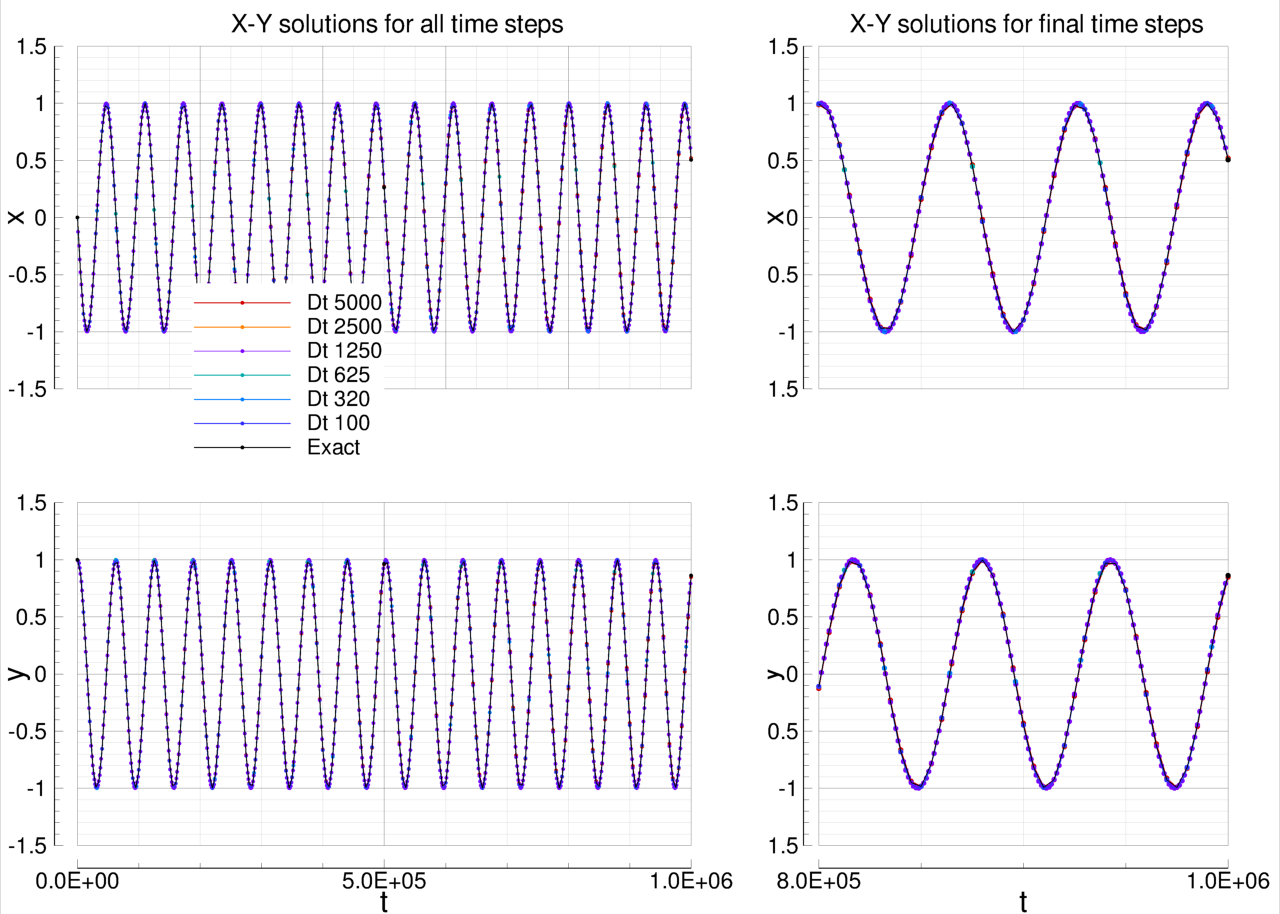
\includegraphics[width=1.00\textwidth]{errors-analysis/oscillation/errors_analysis-oscillation-ls-runge-kutta-5.png}
    \caption{5 stages}\label{fig:results-oscillation-ls-runge-kutta-5}
  \end{subfigure}
  \caption{Oscillation equations solutions computed by means of low storage Runge-Kutta solvers}\label{fig:results-oscillation-ls-runge-kutta-1-5}
\end{figure}

\begin{figure}[!ht]
  \centering
  \begin{subfigure}[b]{0.45\textwidth}
    \centering
    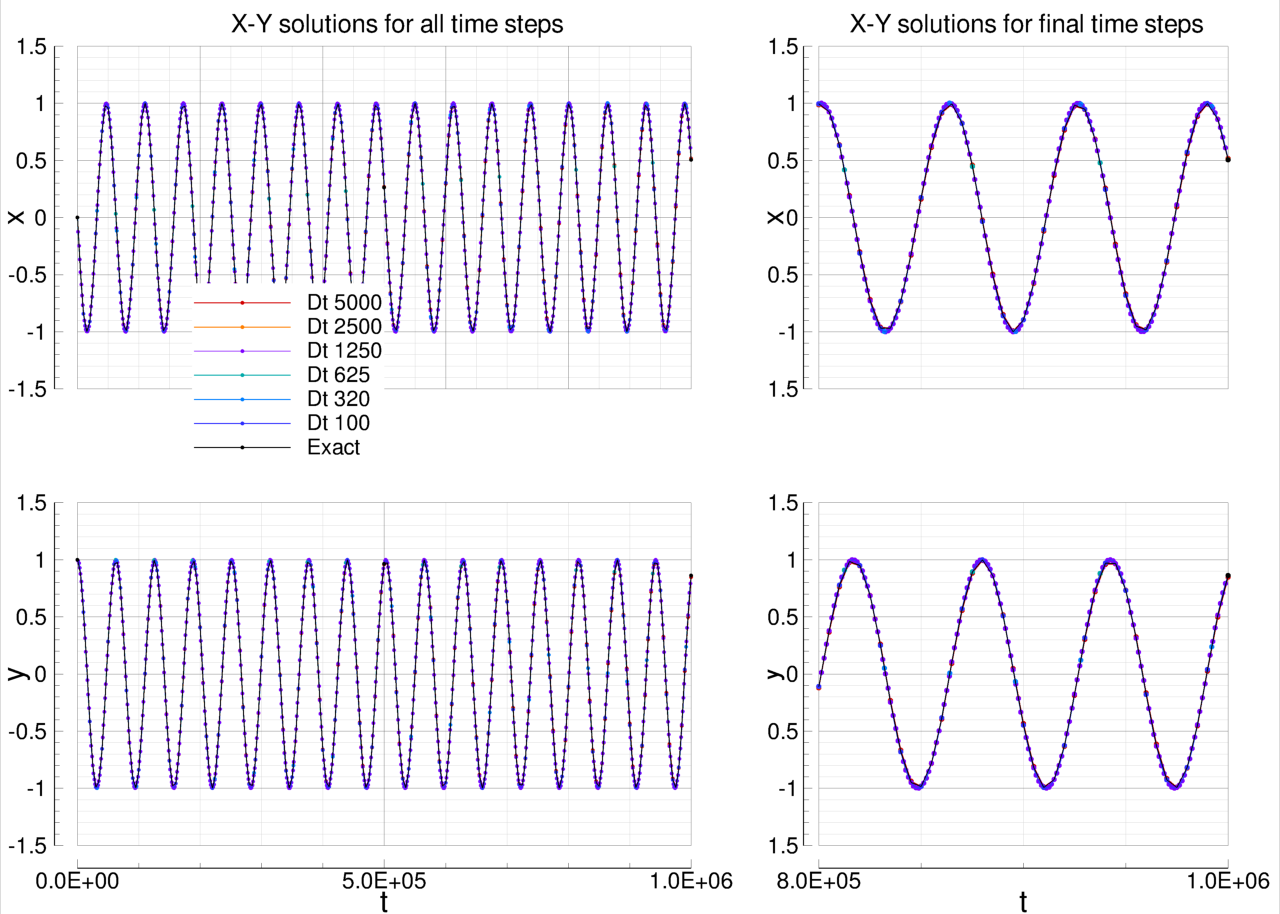
\includegraphics[width=1.00\textwidth]{errors-analysis/oscillation/errors_analysis-oscillation-ls-runge-kutta-6.png}
    \caption{6 stages}\label{fig:results-oscillation-ls-runge-kutta-6}
  \end{subfigure}\quad%
  \begin{subfigure}[b]{0.45\textwidth}
    \centering
    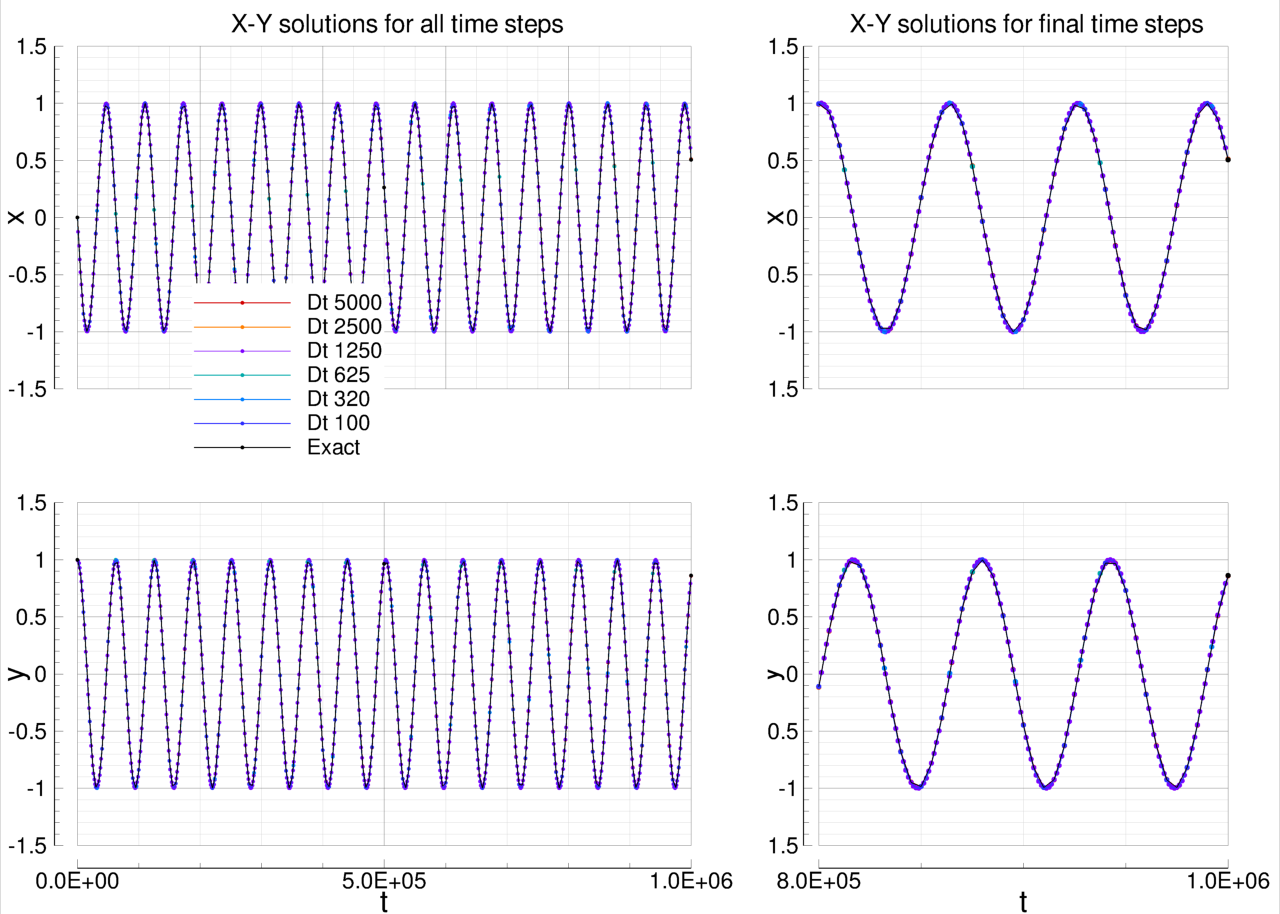
\includegraphics[width=1.00\textwidth]{errors-analysis/oscillation/errors_analysis-oscillation-ls-runge-kutta-7.png}
    \caption{7 stages}\label{fig:results-oscillation-ls-runge-kutta-7}
  \end{subfigure}
  \begin{subfigure}[b]{0.45\textwidth}
    \centering
    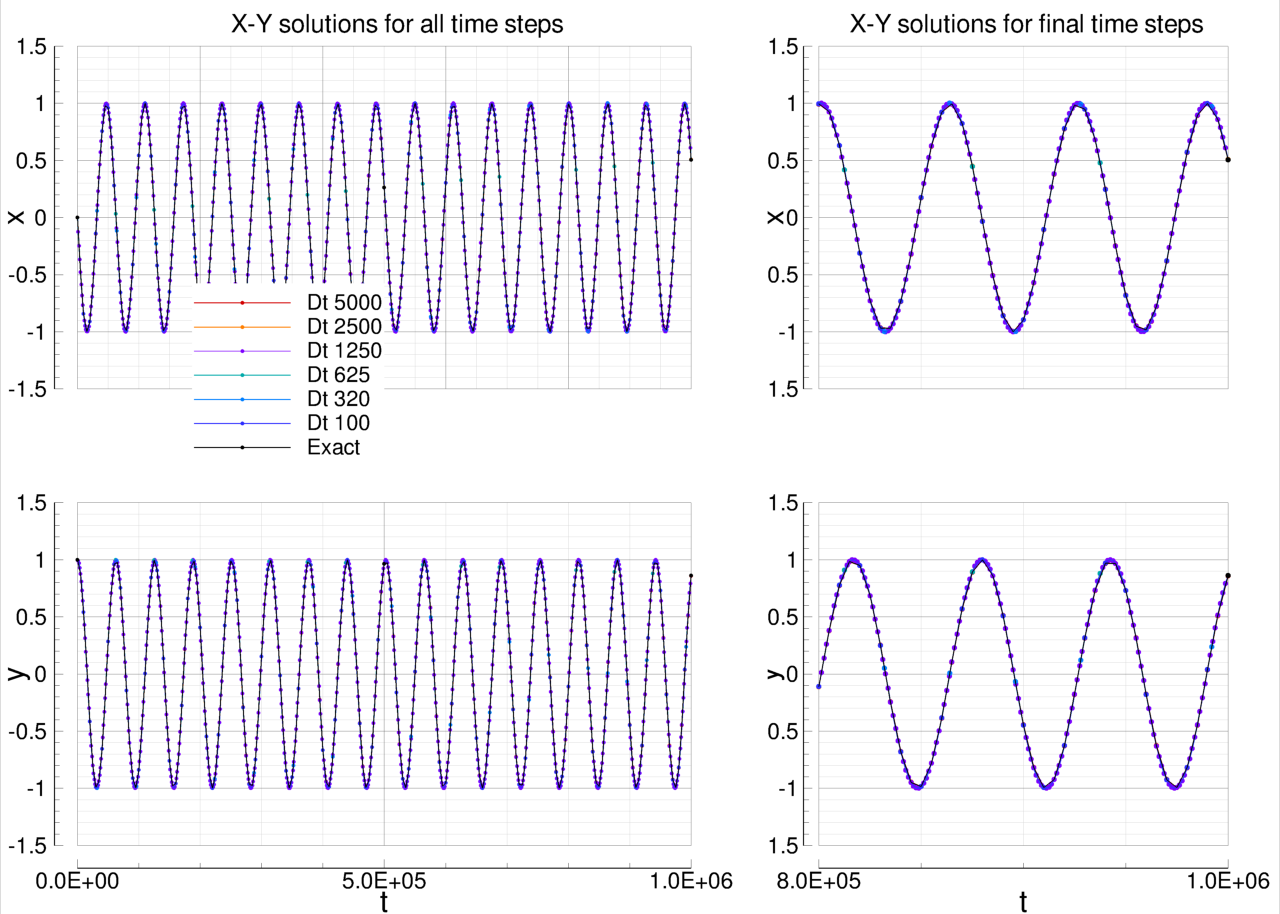
\includegraphics[width=1.00\textwidth]{errors-analysis/oscillation/errors_analysis-oscillation-ls-runge-kutta-12.png}
    \caption{12 stages}\label{fig:results-oscillation-ls-runge-kutta-12}
  \end{subfigure}\quad%
  \begin{subfigure}[b]{0.45\textwidth}
    \centering
    \includegraphics[width=1.00\textwidth]{errors-analysis/oscillation/errors_analysis-oscillation-ls-runge-kutta-13.png}
    \caption{13 stages}\label{fig:results-oscillation-ls-runge-kutta-13}
  \end{subfigure}
  \begin{subfigure}[b]{0.45\textwidth}
    \centering
    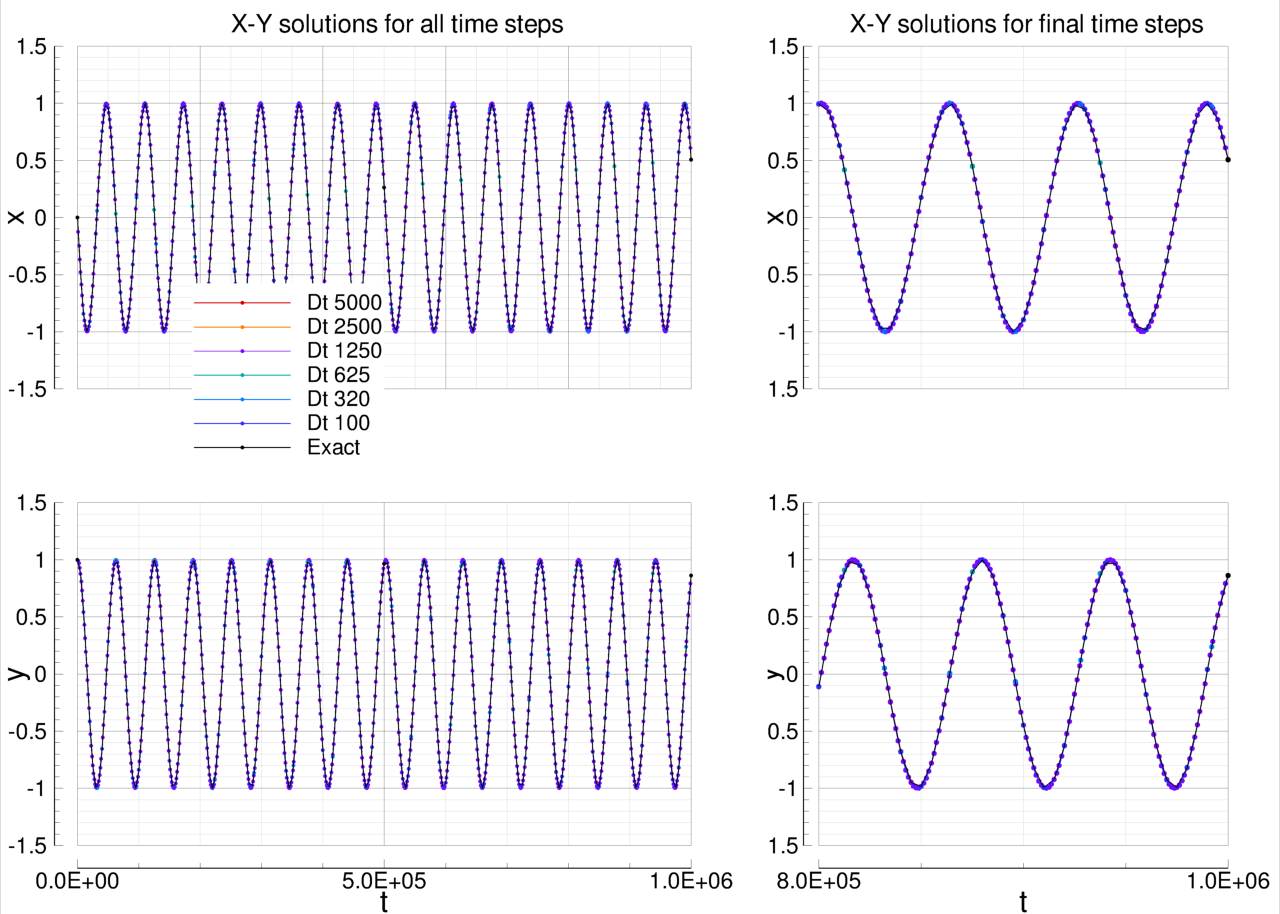
\includegraphics[width=1.00\textwidth]{errors-analysis/oscillation/errors_analysis-oscillation-ls-runge-kutta-14.png}
    \caption{14 stages}\label{fig:results-oscillation-ls-runge-kutta-14}
  \end{subfigure}\quad%
  \caption{Oscillation equations solutions computed by means of low storage Runge-Kutta solvers}\label{fig:results-oscillation-ls-runge-kutta-6-14}
\end{figure}

